%%%%%%%%%%%%%%%%%%%%%%%%%%%%%%%%%%%%%%%%%%%%%%%%%%%%%%%%%
%                                                       %
% La clase: 11pt o 10pt, es un draft o copia definitiva %
% Que tipo de codificacion usa, ...                     %
%                                                       %
%%%%%%%%%%%%%%%%%%%%%%%%%%%%%%%%%%%%%%%%%%%%%%%%%%%%%%%%%
\documentclass[11pt,twoside,a4paper]{book}
\usepackage{fancyhdr}
\usepackage{fancybox}
\usepackage[T1]{fontenc}
\usepackage[utf8]{inputenc}
\usepackage[spanish]{babel}
\usepackage{amsfonts}
\usepackage{latexsym}
\usepackage{graphicx}
\usepackage{floatflt}
\usepackage{epsfig}
\usepackage{subfigure}
\usepackage{mathrsfs}
\usepackage{amssymb}
\renewcommand{\baselinestretch}{1.2}
\title{\Huge Servidor Web Tomcat}
\author{José Manuel Cuevas Muñoz, Daniel Ranchal Parrado, Carlos Romeo Muñoz}
\date{9 de Diciembre 2018}
%%%%%%%%%%%%%%%%%%%%%%%%%%%
%                         %
% Comenzamos el documento %
%                         %
%%%%%%%%%%%%%%%%%%%%%%%%%%%
\begin{document}
\maketitle
%%%%%%%%%%%%%%%%%%%%%%%%%%%
%
% Algunos ajustes previos
%
%%%%%%%%%%%%%%%%%%%%%%%%%%%

\renewcommand\bibname{Bibliografía}
\renewcommand\tablename{Tabla}

\pagenumbering{arabic} \fancyhf{} \pagestyle{fancy}
\fancyhead[LO]{\rightmark} % En las pginas impares, parte izquierda del encabezado, aparecer el nombre de seccin
\fancyhead[RE]{\leftmark} % En las pginas pares, parte derecha del encabezado, aparecer el nombre de captulo
\fancyhead[RO,LE]{\thepage} % Nmeros de pgina en las esquinas de los encabezados
\setlength{\headheight}{14pt}
\renewcommand{\sectionmark}[1]{\markright{{\thesection. #1}}} % Formato para la seccin: N.M. Nombre
%%%
%con esto creamos el ndice
\tableofcontents
\listoffigures
%
% Contenido TRABAJO
%

\chapter{Definición del Sistema}
\section{Objetivos y definición del sistema}
El objetivo que se pretende es hacer pruebas exhaustivas, es decir, hacer un \
benchmarking para calcular el rendimiento del servicio web Tomcat. Para hacer\
este tipo de pruebas, se parte de la siguiente información. El sistema operativo\
bajo el que se están haciendo las pruebas es CentOS, cuyo servidor está \
alojado en Azure.
\newline
Para la instalación de Tomcat, se ha utilizado el servicio de virtualización \
docker para instalarlo de una manera sencilla. Para que el host, es decir, el \
servidor pueda dar el servicio que provee el contenedor de docker, hay que ligar\
el puerto del contenedor en el que está sirviendo Tomcat con el puerto que \
nosotros queramos en el host, aunque los autores de este guión y trabajo hemos \
elegido el 80, el puerto por excelencia para el servidor web.

\section{Servicios y sus posibles resultados}
El servidor web Tomcat nos provee una gran cantidad de utilidades para \
aprovechar al máximo este mismo. La primera y la más importante es el despliegue\
de una página web. Tomcat nos permite hacerlo de manera estática, es decir, \
configurar la aplicación antes de activar este servicio o de manera dinámica, \
que es lo más utilizado para servidores que están en producción.
\newline
Para poder realizar esto de una manera sencilla, Tomcat nos da una herramienta \
llamada "Manager", que cómo se ha comentado antes, se pueden hacer despliegues \
y eliminación (undeploy) de cualquier aplicación web además de darnos una lista \
de las aplicaciones que ya están desplegadas.
\newline
Pero las utilidades de "Manager" no son sólo esas, este gestor nos da la opción \
de poder ver las estadísticas de las sesiones de cualquier aplicación y el \
estado del servidor. Otra de las funcionalidades que tiene, al igual que el \
servidor httpd y apache2, es la posibilidad de trabajar con "Virtual Host".
\newline
Otra característica interesante que nos ofrece Tomcat es la gestión de los \
usuario y los roles en las distintas aplicaciones web. Esto evita que tengamos \
una tabla para cada aplicación web que se tenga. En temas de seguridad, Tomcat \
nos permite la configuración de los certificados SSL/TLS para que nuestra \
página tenga el protocolo https.
\newline
Para este experimento, se distinguirán los siguientes resultados:

\begin{itemize}
  \item \textbf{La carga correcta de las imágenes en un tiempo\
  considerablemente bueno.}
  \item \textbf{La carga correcta de las imágenes en un tiempo pésimo.}
  \item \textbf{La carga parcial de las imágenes.}
  \item \textbf{Fallo del servidor web. Ninguna imágen es servida.}
\end{itemize}


\section{Métricas}
Para poder medir la eficacia y la actuación del servidor web Tomcat se han \
considerado los siguientes parámetros a examinar:

\begin{itemize}
  \item \textbf{Peticiones por segundo}
  \item \textbf{Tiempo por cada grupo de peticiones al mismo tiempo}
  \item \textbf{Tiempo por cada petición}
  \item \textbf{Uso de la CPU}
  \item \textbf{E/S Disco}
  \item \textbf{E/S Red}
\end{itemize}

\pagebreak
\section{Parámetros}
Los parámetros que pueden afectar a la medición del rendimiento del servidor \
web Tomcat son los siguientes:

\begin{itemize}
  \item \textbf{La lejanía con el centro de datos}
  \item \textbf{Los procesos que se ejecutan en segundo plano}
  \item \textbf{Estado de nuestra conexión a Internet}
  \item \textbf{Hardware empleado en el servidor}
\end{itemize}

Para poder mitigar los efectos que producen estos parámetros,la prueba se ejecutará varias veces y se harán los cáculos oportunos para representar de una manera correcta las estadísticas.

\chapter{Evaluación del Sistema}
Definición de la experimentación a realizar. Qu evaluacin se seguir, cual ser la carga de trabajo, qu experimentos se van a realizar y finalmente se analizarn los resultados de la experimentacin.

\section{Tcnicas de evaluacin}
Qu tcnica de evaluacin se seguir.

\section{Carga de trabajo}
Cual ser la carga de trabajo, en qu consiste.

\section{Diseo de Experimentos}
Cmo se han diseado los experimentos. En qu consiste la experimentacin a realizar.

\section{Anlisis de los resultados}
Estudio y anlisis de los resultados provenientes de la experimentacin. Tablas y grficas con los datos (se requiere un nmero suficiente de muestras resultado de la experimentacin)

\chapter{Conclusiones y discusión}

En primer lugar, se aprecia un fuerte problema en el hardware de este servidor \
debido al cuello de botella que aparece al ejecutar los bencharmarks en la CPU, \
esto es fácil de comprender, debido a que la concurrencia toma protagonismo en \
estos tests, con algunos fijándola en valores como 10 peticiones concurrentes. \
Esta teoría es afirmada por las gráficas mostradas, donde vemos fácilmente como \
el procesador llega a funcionar a niveles cercanos al 100\% de utilidad durante \
la duración de las pruebas efectuadas.

\begin{figure}
   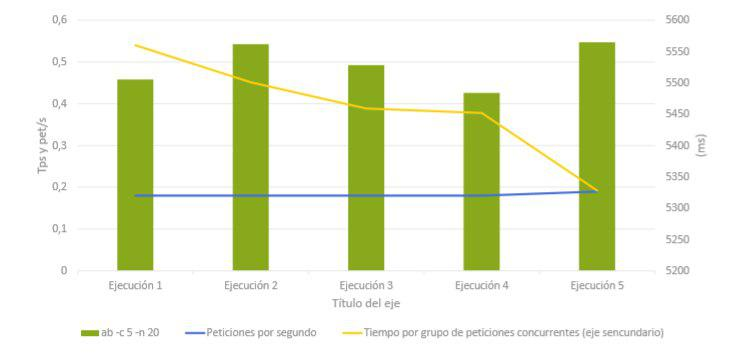
\includegraphics[width=\textwidth]{grafica1.jpg}
   \caption{Uso de CPU}
   \label{cpu}
\end{figure}

Además de esto, otro factor determinante en este caso es el bajo número de \
transferencias por segundo que el servidor es capaz de aguantar y que está \
fuertemente relacionado con el almacenamiento del mismo en el cual se almacenan \
las fotografías que sirven como cargas de prueba, el cual en ninguna prueba es \
capaz de llegar ni tan siquiera a la unidad, y eso es algo que los encargados \
de testear su funcionamiento hemos conocido de primera mano al tener que \
esperar grandes cantidades de tiempo a que todos los tests fueran completados \
varias veces con éxito. En cuanto a las peticiones por segundo, casi nunca \
superan el cuarto de unidad, hecho que no hace más que corroborar las \
afirmaciones anteriores. \newline

\begin{figure}
   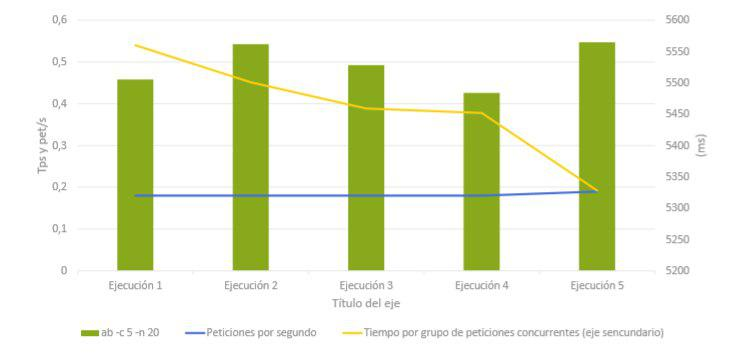
\includegraphics[width=\textwidth]{grafica1.jpg}
   \caption{Transferencias por Segundo, peticiones por segundo \
   y tiempo empleado en un grupo de peticiones concurrentes.}
   \label{Fig1}
\end{figure}

Si contemplamos el gráfico \ref{Fig1}, nos damos cuenta de que el número de \
peticiones por segundo, al ser un parámetro íntimamente ligado al hardware \
sobre el que se esté ejecutando el banco de pruebas escogido, apenas varía, \
puesto que la CPU solo es capaz de ejecutar un número determinado de ellas, \
siendo todas iguales. Lo interesante de este gráfico, es ver como el tiempo \
empleado en servir un grupo de peticiones concurrentes decae a lo largo de las \
cinco ejecuciones del test. Tras indagar en los motivos de este aumento del \
rendimiento, nos damos cuenta de que Azure es un servicio de computación en la \
nube que alardea de proveer de una caché inteligente a sus máquinas virtuales \
que estén corriendo en sus servidores, como es nuestro caso, eso por ello por \
lo que se aprecia esta mejora en el rendimiento, debido a que gran parte de los \
datos que son necesarios para la ejecución de la prueba, ya están cargados en \
la caché del servidor y son accesibles de manera mucho más rápida para la \
siguiente ejecución. \newline

Si contemplamos las gráficas \ref{Fig2}, \ref{Fig3} y \ref{Fig4}, no hay gran \
diferencia entre ellas en cuanto al parámetro de medición, el número de \
transferencias por segundo del disco del servidor. Para analizar las gráficas, \
recordemos que estos datos han sido tomados con el monitor sar, mientras que ab \
era ejecutado, tras ello, se ha realizado la media aritmética de los valores \
del parámetro interesado que sar tomaba cada 10 segundos durante la ejecución \
del test. Entonces, podemos ver como apenas hay diferencias significativas \
entre las ejecuciones, por ejemplo, en la gráfica \ref{Fig2}, vemos como\
normalmente el test de menor concurrencia y menos repeticiones\
(línea amarilla), tarda normalmente menos tiempo que el test con más \
concurrencia y el doble de repeticiones (línea verde), aunque veamos \
ejecuciones donde estas posiciones se inviertan, esto se debe más al margen de \
error que a otra cosa. En cuanto a la gráfica \ref{Fig4}, la referida a los \
resultados del mosaico de imágenes pequeñas, observamos como la línea azul, \
la correspondiente con el uso de https, lo cual es curioso debido a que en las \
dos últimas pruebas se habían mantenido por debajo, sin embargo, no es de \
preocupación, ya que no se aprecian diferencias muy significativas en la \
mayoría de las ejecuciones, sin embargo, vemos como esa línea sube hasta una \
transferencia por segundo en la segunda ejecución, lo cual es muy significativo.
La imagen general de estas pruebas es que mientras más grandes sean las \
imágenes del banco de pruebas, menos transferencias por segundo se llevarán a \
cabo, lo cual es lógico, puesto que son archivos más grandes. \newline

\begin{figure}
   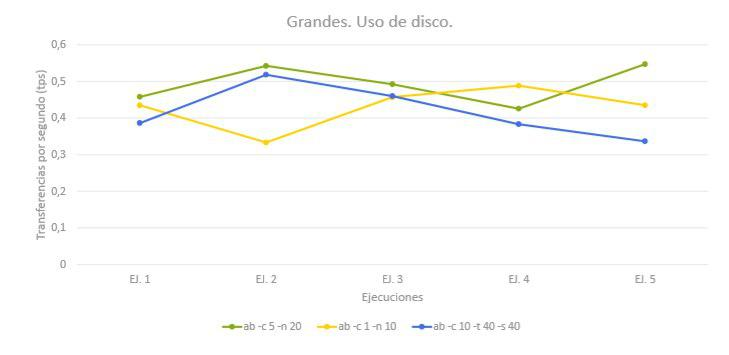
\includegraphics[width=\textwidth]{grafica2.jpg}
   \caption{Uso de disco en las cinco ejecuciones con imágenes grandes}
   \label{Fig2}
\end{figure}
\begin{figure}
   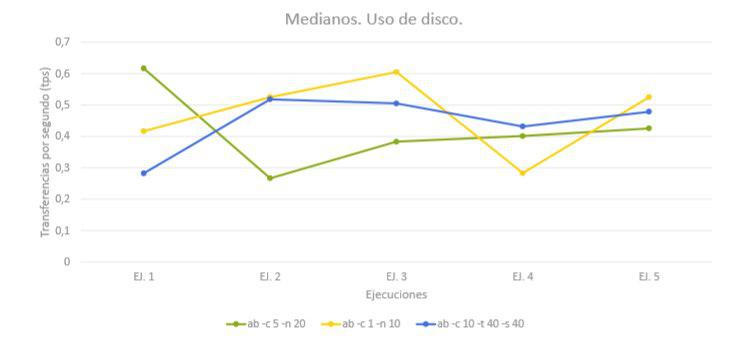
\includegraphics[width=\textwidth]{grafica3.jpg}
\caption{Uso de disco en las cinco ejecuciones con imágenes medianas}   \label{Fig3}
\end{figure}
\begin{figure}
   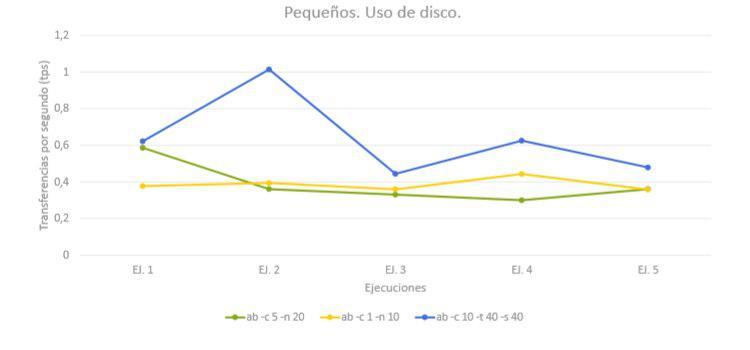
\includegraphics[width=\textwidth]{grafica4.jpg}
   \caption{Uso de disco en las cinco ejecuciones con imágenes pequeñas}
   \label{Fig4}
\end{figure}

Si analizamos ahora el uso de la red del servidor, aquí no tenemos ningún \
problema de cuello de botella, Azure nos proporciona una velocidad de conexión \
veloz y estable y no es algo que un administrador de un servidor pequeño como \
este tenga que preocuparse, por supuesto, mientras más exigente sea el test con \
la CPU, lo será con el uso de red que éste requerirá, puesto que estamos \
hablando de un servidor web. \newline

\begin{figure}
   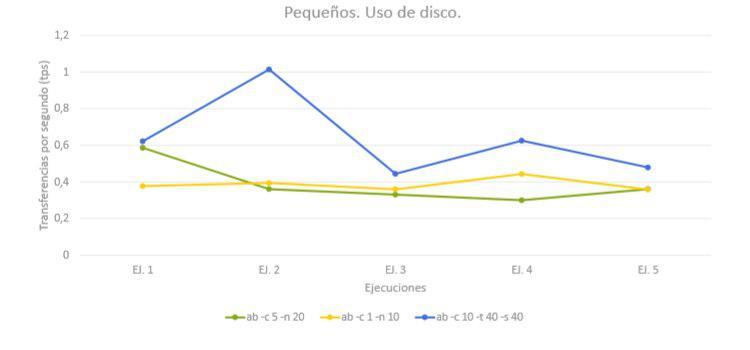
\includegraphics[width=\textwidth]{grafica4.jpg}%mete aqui tu foto
   \caption{Uso de Red}
   \label{Fig5}
\end{figure}

En conclusión, hemos detectado que nuestro cuello de botella es una CPU que a \
pesar de ser muy potente en el conjunto de todos sus núcleos, apenas aguantaría \
un servidor web pequeño como este ante un importante número de peticiones al \
servidor, esto es debido a que la cuenta de estudiante de Microsoft Azure que \
estamos empleando para este trabajo solo ofrece un núcleo de procesador, \
potente, si, pero que flaquea en tareas que involucren una alta concurrencia \
de peticiones. Y es que ese es el argumento por el cual los procesadores \
empleados para su uso en servidores de cualquier tipo suelen contar con un \
gran número de núcleos tanto físicos como lógicos y poder procesar rápidamente \
todas las peticiones que reciba. En cuanto a la referenciación, sabemos que los \
resultados aquí mostrados corresponden con los de un servidor de \
especificaciones limitadas, útil para este propósito, pero de limitado uso, y \
es que, tras haber ejecutado numerosos bancos de pruebas centrados en multitud \
de aspectos de un sistema informático, entre ellos Apache Benchmark, hemos \
encontrado que fácilmente, un ordenador doméstico con todos sus núcleos \
activados puede sobrepasar fácilmente el rendimiento de este procesador, \
organizaciones como SPEC tienen precisamente esa función, la de examinar este \
tipo de equipos informáticos para poder realizar comparativas, lo cual nos es \
muy útil a la hora de sacar conclusiones sobre el desempeño de este hardware. \
Por último, hemos de decir, que Microsoft Azure es una útil herramienta para \
alojar cualquier tipo de servidor o aplicación web y que nos ha sido muy útil \
para la realización de este trabajo y que, previo pago de la capacidad \
necesaria, se puede obtener muchísima potencia de cómputo de ella.


%\section{Cuestiones}

%% APENDICES
%\ \newpage
\appendix

\renewcommand{\baselinestretch}{1.2}

% BIBLIOGRAFIA
\bibliography{biblio}
\bibliographystyle{unsrt}
\cite{KM2000}
\end{document}
